\section{Compact Muon Solenoid}
\label{ch:cms}

The Compact Muon Solenoid (CMS) detector is 
designed to measure $pp$ collisions from the LHC.
CMS is installed 100 m underground near the French village
of Cessy.  CMS is barrel-shaped and stretches roughly 25 m long with
a diameter of roughly 15 m.  It weighs 12,500 tons.
A schematic of CMS is shown in Figure \ref{fig:cms}.

\begin{figure}
  \centering
  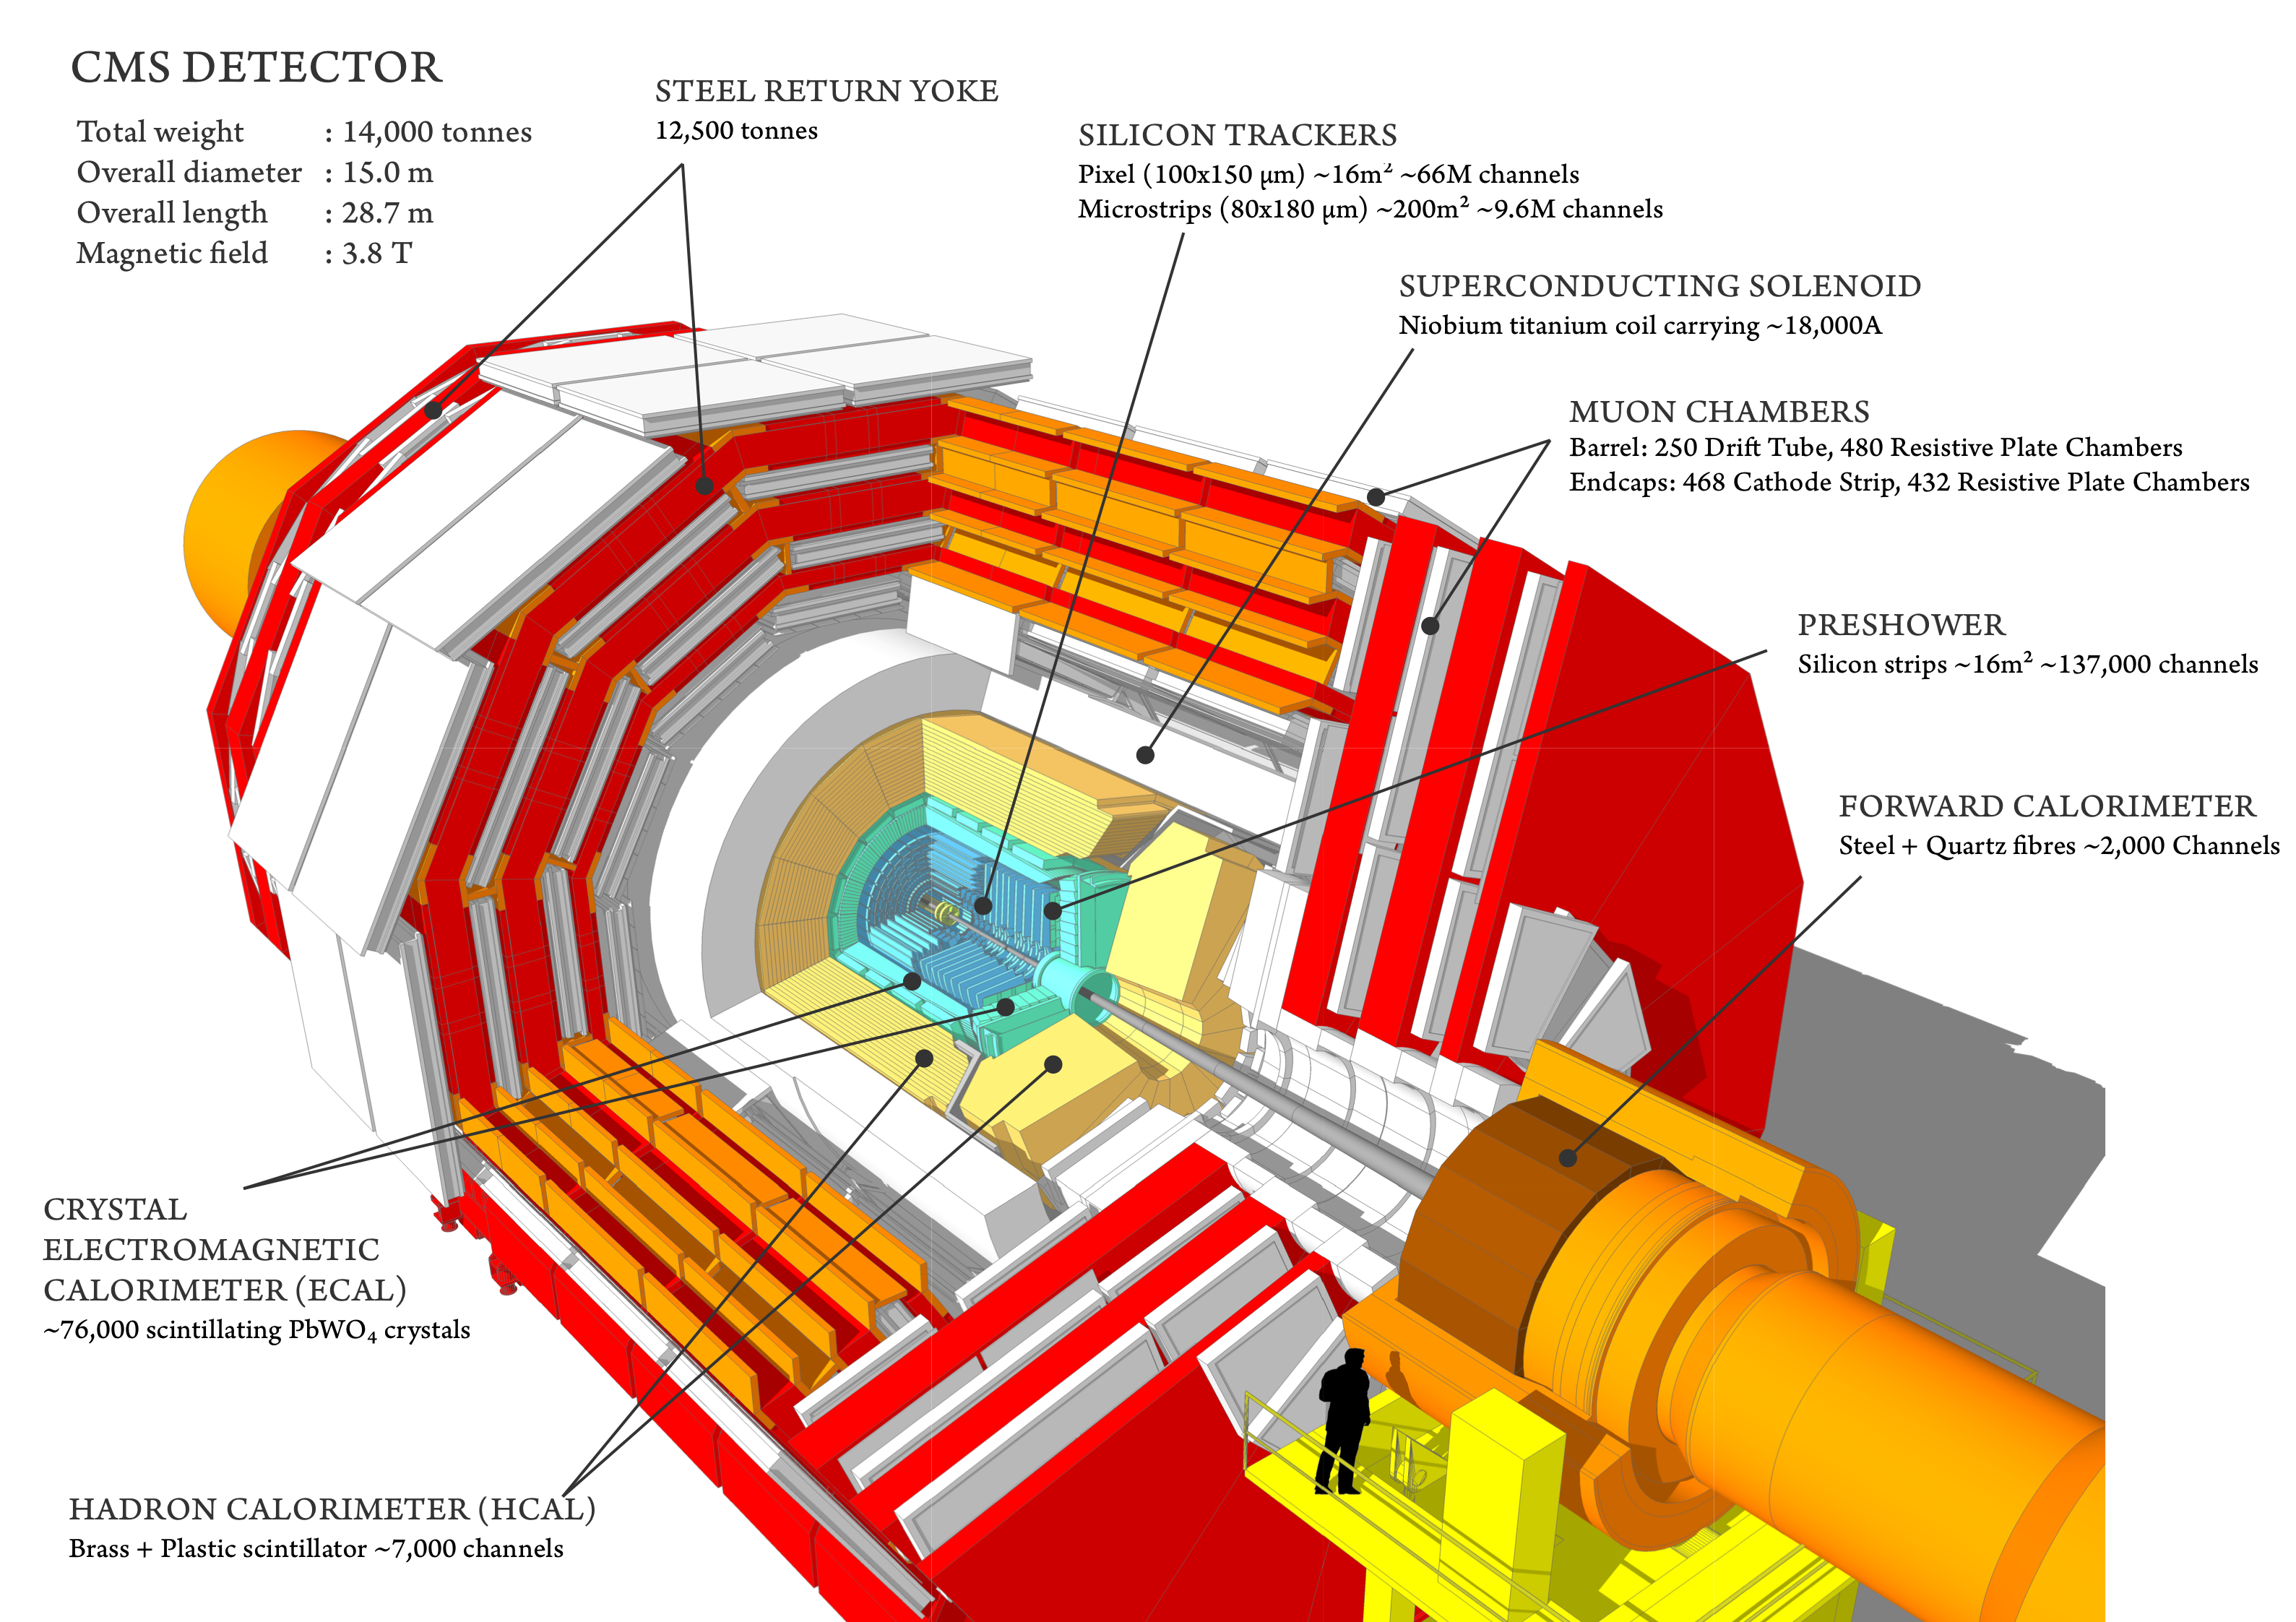
\includegraphics[width=\textwidth]{tex/cms/fig/cms.png}
  \caption{A cartoon schematic of the CMS detector}
  \label{fig:cms}
\end{figure}

CMS is designed to operate in a very challenging environment.
The total $pp$ cross section for collisions with 
beam energy of 7 TeV is expected to be about 100 mb.
The LHC design luminosity is $10^{34}\text{cm}^{-2}\text{s}^{-1}$, which
corresponds to a collision rate of $10^9$ collisions per second.
Furthermore, in addition to the $pp$ interaction of interest,
20 inelastic $pp$ collisions will take place in the same
bunch crossing (an effect known as ``pile-up'').  
In total, at design luminosity, roughly 1000 charged particles 
will be produced at the interaction region every 25 ns.
This large flux of particles from the interaction region leads to
high radiation levels, which can impact the performance of the detector and front-end electronics.
In addition, charged particles from pile-up
interactions may be confused with charged particles from the interaction
of interest.  This effect can be ameliorated somewhat by using
high granularity detectors with good timing resolution (and therefore low occupancy).

The detector requirements for CMS may be summarized as follows:
\begin{itemize}
  \item Good muon identification and momentum resolution over
    a wide range of momenta and angles, good dimuon mass resolution
    ($\approx 1\%$ at 100 GeV), and the ability to determine 
    unambiguously the charge of muons with $p < 1$ TeV.
  \item Good charged particle momentum resolution and reconstruction
    efficiency in the inner tracker.  Efficient triggering and offline
    tagging of $\tau$'s and $b$-jets, requiring pixel detectors close
    to the interaction region.
  \item Good electromagnetic energy resolution, good diphoton and dielectron
    mass resolution ($\approx 1\%$ at 100 GeV), wide geometric coverage,
    $\pi^0$ rejection, and efficient photon and lepton isolation at high
    luminosities.
  \item Good resolution of the imbalance of the total energy measured in the transverse plane
    and good dijet-mass resolution, requiring hadron calorimeters with a large hermetic
    geometric coverage and fine lateral segmentation.
\end{itemize}

The design of the CMS detector is described in this section, and it meets these requirements.  
Unless otherwise stated, all of the information in this section comes from References
\cite{cms-jinst} and \cite{cms-tdr}.

